\documentclass[conference]{IEEEtran}
\IEEEoverridecommandlockouts
\usepackage{cite}
\usepackage{amsmath,amssymb,amsfonts}
\usepackage{algorithmic}
\usepackage{graphicx}
\usepackage{textcomp}
\usepackage{xcolor}
\usepackage{booktabs}
\usepackage{multirow}
\usepackage{url}
\usepackage{tikz}
\usetikzlibrary{arrows.meta, positioning, shapes.geometric, calc, fit, backgrounds}
\def\BibTeX{{\rm B\kern-.05em{\sc i\kern-.025em b}\kern-.08em
    T\kern-.1667em\lower.7ex\hbox{E}\kern-.125emX}}
\begin{document}

\title{BioVerse: An AI-Assisted Biologically-Constrained DNA Data Encoding System with Integrated Integrity Verification}

\author{\IEEEauthorblockN{1\textsuperscript{st} Dr. K. Vijayalakshmi}
\IEEEauthorblockA{\textit{Dept. of Computational Intelligence} \\
\textit{(of Affiliation)}\\
\textit{SRM Institute of Science \& Technology}\\
Kattankulathur, Tamil Nadu \\
vijaylak@srmist.edu.in}
\and
\IEEEauthorblockN{2\textsuperscript{nd} Momin Nisar Zargar}
\IEEEauthorblockA{\textit{Dept. of Computational Intelligence} \\
\textit{(of Affiliation)}\\
\textit{SRM Institute of Science \& Technology}\\
Kattankulathur, Tamil Nadu \\
mz0343@srmist.edu.in}
\and
\IEEEauthorblockN{3\textsuperscript{rd} Safwan Sajad Thokar}
\IEEEauthorblockA{\textit{Dept. of Computational Intelligence} \\
\textit{(of Affiliation)}\\
\textit{SRM Institute of Science \& Technology}\\
Kattankulathur, Tamil Nadu \\
st0578@srmist.edu.in}
}

\maketitle

\begin{abstract}
DNA is being explored as a long-term storage medium because it is extremely dense and stable for centuries. A practical DNA storage system, however, must do three things at the same time: (i) produce DNA strings that real laboratories can actually synthesise, (ii) protect the stored data from corruption and tampering, and (iii) be measured in a way that lets different systems be compared fairly. Most existing systems address only one of these concerns. This paper presents \textbf{BioVerse}, a complete DNA data storage pipeline that addresses all three. We introduce a simple ``rotation'' rule that turns binary data into DNA while keeping the resulting strand within standard biological limits (no long single-base runs, balanced GC content, and no common restriction enzyme sites), and we prove the rule is fully reversible. We also propose a dual-purpose watermark: an AI-generated DNA fingerprint that both camouflages the data and carries a hash-based integrity tag, removing the need for an external checksum file. Finally, we provide a benchmark suite that measures storage density, security, error resilience, biological realism, and runtime in one place. On test inputs from 128\,B to 64\,KB, BioVerse achieves 100\% biological compliance (longest single-base run drops from 9 to 3, all five tested restriction sites are removed) with only a 2.31\% rotation rate, recovers data losslessly, tolerates up to 0.5\% random base substitutions through Reed-Solomon coding, and detects every one of 50 single-base tampering attempts.
\end{abstract}

\begin{IEEEkeywords}
DNA data storage, biological constraints, AES encryption, Reed-Solomon error correction, LSTM, watermarking, integrity verification
\end{IEEEkeywords}

\section{Introduction}

The amount of digital data created every year now grows much faster than traditional disk and tape technologies can keep up with for long-term archival. DNA has attracted attention as an alternative because, in principle, it can store about two bits in every nucleotide and remain readable for hundreds of years if kept dry and cool \cite{b1}. Several research groups have already shown that arbitrary files can be written into synthetic DNA and read back \cite{b2,b3,b4}.

Moving from these proofs of concept to a usable system, however, raises three practical problems:

\begin{enumerate}
\item \textbf{The DNA must be synthesisable.} Real laboratories cannot reliably make strands that contain long stretches of the same base, very high or very low GC content, or sequences that look like cut sites for common restriction enzymes \cite{b5}.
\item \textbf{The data must be protected.} Most existing systems store the integrity check (a hash or manifest) in a separate file, so an attacker who can change the DNA can usually change the checksum too.
\item \textbf{Different systems should be comparable.} Today every paper reports its own subset of metrics, which makes it hard to tell whether a new method is genuinely better.
\end{enumerate}

This paper presents \textbf{BioVerse}, an end-to-end pipeline that addresses all three problems together. Our contributions are:

\begin{itemize}
\item \textbf{A constraint-aware encoder.} A simple rotation rule converts binary data into DNA while guaranteeing no run of more than three identical bases, GC content between 30\% and 70\% in every 20-base window, and no occurrence of five common restriction sites. The rule is fully reversible; nothing is lost.
\item \textbf{A dual-purpose AI watermark.} An LSTM- (or Markov-) generated DNA fingerprint both makes the strand look more natural and carries a SHA-256-derived tag, so tamper detection no longer needs a separate file.
\item \textbf{A reproducible benchmark.} A single script measures storage density, encryption strength, Reed-Solomon resilience, biological realism, and runtime, and emits IEEE-ready tables.
\end{itemize}

The rest of the paper is organised as follows. Section~II compares BioVerse with prior DNA storage systems. Section~III describes the pipeline. Section~IV explains how we evaluate it. Section~V covers the implementation. Section~VI reports the measurements. Section~VII discusses honest limitations, and Section~VIII concludes.

\section{Related Work}

Table~\ref{tab:related} summarizes existing DNA data storage systems and their capabilities compared to BioVerse.

\begin{table}[htbp]
\caption{Comparison of DNA Data Storage Systems}
\begin{center}
\setlength{\tabcolsep}{3pt}
\renewcommand{\arraystretch}{1.1}
\resizebox{\columnwidth}{!}{%
\begin{tabular}{|l|c|c|c|c|}
\hline
\textbf{System} & \textbf{Density} & \textbf{Constr.} & \textbf{Integrity} & \textbf{ECC} \\
 & \textbf{(bits/nt)} & & & \\
\hline
Church \cite{b2} & 1.00 & None & External & None \\
\hline
Goldman \cite{b3} & 1.58 & HP & External & 4$\times$ \\
\hline
Grass \cite{b6} & 1.14 & None & External & RS \\
\hline
Erlich \cite{b4} & 1.98 & Screened & External & LT \\
\hline
Organick \cite{b7} & $\sim$1.10 & None & External & XOR \\
\hline
\textbf{BioVerse} & \textbf{1.33--1.75\textsuperscript{a}} & \textbf{HP+GC+RE} & \textbf{Embedded} & \textbf{RS-32} \\
\hline
\end{tabular}}
\\[2pt]
{\footnotesize\raggedright
\textsuperscript{a}Measured on 128\,B--64\,KB inputs after AES-128 expansion and 32-byte RS parity.\\
HP = Homopolymer, GC = GC-balance, RE = Restriction enzyme avoidance.\\
RS = Reed-Solomon, LT = Luby Transform.\par}
\label{tab:related}
\end{center}
\end{table}

Church et al.\ \cite{b2} demonstrated the first large-scale DNA archive but used a one-bit-per-base mapping and ignored synthesis limits such as long single-base runs. Goldman et al.\ \cite{b3} added a rotating ternary code that avoids those runs and reaches 1.58 bits/nt, but did not control GC content or restriction sites. Grass et al.\ \cite{b6} added Reed-Solomon error correction to silica-encapsulated DNA, again without enforcing biological rules on the sequence itself.

Erlich and Zielinski \cite{b4} pushed density to almost the theoretical maximum (1.98 bits/nt) using DNA Fountain codes, by generating many candidate strands and discarding any that violate biological rules. The approach is effective but wasteful, because rejected strands are simply thrown away. Organick et al.\ \cite{b7} showed how to do random access in a large-scale DNA archive but again did not enforce sequence-level constraints.

Yazdi et al.\ \cite{b5} provided the theoretical foundations of constrained coding for DNA, but the work stopped short of a full deployable system.

BioVerse differs from this prior work in three concrete ways: (i) it enforces \emph{three biological rules at once} (run length, GC balance, and restriction-site avoidance) using a deterministic rotation step instead of trial-and-error rejection; (ii) it places the integrity check \emph{inside the DNA itself}, so there is no separate file an attacker can attack independently; and (iii) it ships with a single benchmark script that lets future systems be compared on identical metrics.

\section{System Architecture}

The BioVerse encoder is a six-stage pipeline. A user file is first encrypted, then protected with error-correcting parity, then mapped to DNA under biological constraints, and finally combined with an AI-generated fingerprint that carries a tamper tag. The decoder applies the same steps in reverse. In compact form,

\begin{equation}
\text{File} \xrightarrow{\text{AES}} \text{ciphertext} \xrightarrow{\text{RS}} \text{ECC bytes} \xrightarrow{\text{2 bits/base}} \text{DNA}_c \to \text{.dna file}
\label{eq:pipeline}
\end{equation}

\noindent and Fig.~\ref{fig:pipeline} shows the full data flow, including the small ``rotation flag'' sideband that makes the constrained step exactly reversible and the AI fingerprint that carries the integrity tag.

\begin{figure*}[t]
\centering
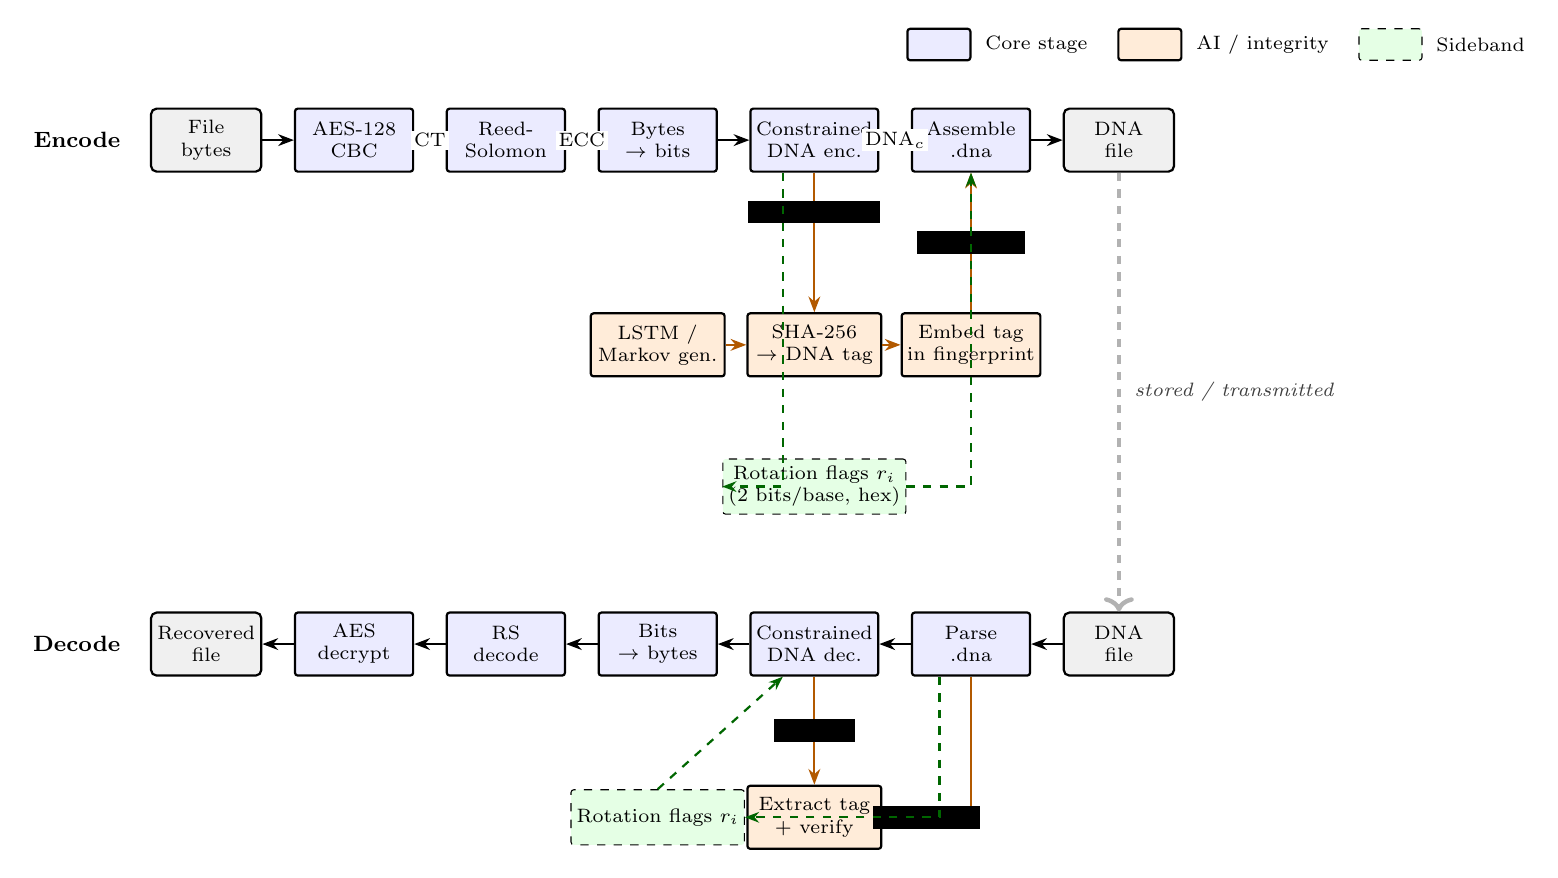
\begin{tikzpicture}[
    font=\scriptsize,
    every node/.style={inner sep=2pt},
    stage/.style={draw, rounded corners=1pt, minimum height=8mm, minimum width=15mm,
                  align=center, fill=blue!8, thick},
    ai/.style={draw, rounded corners=1pt, minimum height=8mm, minimum width=17mm,
               align=center, fill=orange!15, thick},
    io/.style={draw, rounded corners=2pt, minimum height=8mm, minimum width=14mm,
               align=center, fill=gray!12, thick},
    sideband/.style={draw, dashed, rounded corners=1pt, minimum height=7mm,
                     minimum width=22mm, align=center, fill=green!10},
    flow/.style={-{Stealth[length=2mm]}, thick},
    aiflow/.style={-{Stealth[length=2mm]}, thick, orange!70!black},
    side/.style={-{Stealth[length=1.8mm]}, thick, dashed, green!40!black},
    edgelbl/.style={font=\scriptsize, fill=white, inner sep=1pt},
    rowlbl/.style={font=\footnotesize\bfseries, anchor=east},
]

% --------- Encode row (y = 0) ----------
\node[io]                         (file)     at ( 0.0, 0) {File\\bytes};
\node[stage, right=4mm of file]   (aes)                   {AES-128\\CBC};
\node[stage, right=4mm of aes]    (rs)                    {Reed-\\Solomon};
\node[stage, right=4mm of rs]     (bin)                   {Bytes\\$\to$ bits};
\node[stage, right=4mm of bin]    (cenc)                  {Constrained\\DNA enc.};
\node[stage, right=4mm of cenc]   (assemble)              {Assemble\\.dna};
\node[io,    right=4mm of assemble] (dnafile)             {DNA\\file};

\node[rowlbl] at ($(file.west)+(-3mm,0)$) {Encode};

% Encode arrows with labels above
\draw[flow] (file)     -- (aes);
\draw[flow] (aes)      -- node[edgelbl]{CT}              (rs);
\draw[flow] (rs)       -- node[edgelbl]{ECC}             (bin);
\draw[flow] (bin)      -- (cenc);
\draw[flow] (cenc)     -- node[edgelbl]{$\text{DNA}_c$}  (assemble);
\draw[flow] (assemble) -- (dnafile);

% --------- AI branch (y = -2.6) ----------
\node[ai] (lstm)  at ($(bin   |- 0,-2.6)$)        {LSTM /\\Markov gen.};
\node[ai] (hash)  at ($(cenc  |- lstm)$)          {SHA-256\\$\to$ DNA tag};
\node[ai] (embed) at ($(assemble |- lstm)$)       {Embed tag\\in fingerprint};

\draw[aiflow] (lstm)  -- (hash);
\draw[aiflow] (hash)  -- (embed);
% payload -> hash
\draw[aiflow] (cenc.south) -- ++(0,-0.5) -| (hash.north)
      node[pos=0.25, edgelbl, black]{payload hash};
% embedded fingerprint -> assemble
\draw[aiflow] (embed.north) -- (assemble.south)
      node[midway, edgelbl, black]{fingerprint};

% --------- Sideband (y = -4.4) ----------
\node[sideband] (rot) at ($(cenc |- 0,-4.4)$) {Rotation flags $r_i$\\(2 bits/base, hex)};
\draw[side] (cenc.south) ++(-4mm,0) |- (rot.west);
\draw[side] (rot.east) -| (assemble.south);

% --------- Decode row (y = -6.4) ----------
\node[io]                          (rec)      at (0.0, -6.4) {Recovered\\file};
\node[stage, right=4mm of rec]     (daes)                    {AES\\decrypt};
\node[stage, right=4mm of daes]    (drs)                     {RS\\decode};
\node[stage, right=4mm of drs]     (dbin)                    {Bits\\$\to$ bytes};
\node[stage, right=4mm of dbin]    (dcenc)                   {Constrained\\DNA dec.};
\node[stage, right=4mm of dcenc]   (parse)                   {Parse\\.dna};
\node[io,    right=4mm of parse]   (dnafile2)                {DNA\\file};

\node[rowlbl] at ($(rec.west)+(-3mm,0)$) {Decode};

\draw[flow] (dnafile2) -- (parse);
\draw[flow] (parse)    -- (dcenc);
\draw[flow] (dcenc)    -- (dbin);
\draw[flow] (dbin)     -- (drs);
\draw[flow] (drs)      -- (daes);
\draw[flow] (daes)     -- (rec);

% Verifier and decode-side sideband
\node[ai]       (verify) at ($(dcenc |- 0,-8.6)$) {Extract tag\\$+$ verify};
\node[sideband] (rot2)   at ($(dbin  |- verify)$) {Rotation flags $r_i$};

\draw[aiflow] (parse.south) |- (verify.east)
      node[pos=0.75, edgelbl, black]{fingerprint};
\draw[aiflow] (dcenc.south) -- (verify.north)
      node[midway, edgelbl, black]{payload};
\draw[side] (parse.south) ++(-4mm,0) |- (rot2.east);
\draw[side] (rot2.north) -- ($(dcenc.south)+(-4mm,0)$);

% Storage boundary: connect the two .dna file artifacts
\draw[->, ultra thick, gray!60, dashed] (dnafile.south) -- (dnafile2.north)
      node[midway, right=1mm, gray!50!black, font=\scriptsize\itshape]{stored / transmitted};

% --------- Legend (top-right corner) ----------
\begin{scope}[shift={($(dnafile.north east)+(-30mm,8mm)$)}]
  \node[stage,    minimum width=8mm, minimum height=4mm] (lg1) at (0,0) {};
  \node[right=1mm of lg1, font=\scriptsize] (lg1t) {Core stage};
  \node[ai,       minimum width=8mm, minimum height=4mm, right=3mm of lg1t] (lg2) {};
  \node[right=1mm of lg2, font=\scriptsize] (lg2t) {AI / integrity};
  \node[sideband, minimum width=8mm, minimum height=4mm, right=3mm of lg2t] (lg3) {};
  \node[right=1mm of lg3, font=\scriptsize] {Sideband};
\end{scope}

\end{tikzpicture}
\caption{BioVerse end-to-end pipeline. Top row (\emph{Encode}): file $\to$ AES-128 $\to$ Reed-Solomon $\to$ constrained DNA encoder $\to$ assembled \texttt{.dna} file. Bottom row (\emph{Decode}): mirrored inverse pipeline. The green dashed sideband carries the rotation flags $r_i$, making the constrained encoder exactly invertible. The orange branch shows the dual-purpose AI fingerprint: an LSTM/Markov-generated DNA sequence carries the SHA-256-derived integrity tag of the payload, providing both biological camouflage and tamper detection in one field. The vertical dashed link between the two \texttt{.dna~file} artifacts represents the storage / transmission boundary.}
\label{fig:pipeline}
\end{figure*}

\subsection{Encryption Layer}

The input file is encrypted with AES-128 in CBC mode using PKCS7 padding. Each encryption uses a fresh random 16-byte initialisation vector (IV), which is prepended to the ciphertext so the decoder can recover it. With a 128-bit key, brute-force attack at $10^9$ keys per second would take on the order of $10^{21}$ years, so we treat the encryption layer as computationally secure.

\subsection{Error Correction Layer}

The ciphertext is then passed through a Reed-Solomon encoder with 32 parity bytes per 255-byte block. With this configuration the decoder can correct up to 16 byte errors per block and detect up to 32, which is enough headroom to absorb the kinds of point mutations and short read errors that DNA storage typically suffers from.

\subsection{Biologically-Constrained DNA Encoding}

The error-protected ciphertext is a stream of bits, and the encoder turns every two bits into one DNA base. The naive mapping is $00\!\to\!A$, $01\!\to\!T$, $10\!\to\!G$, $11\!\to\!C$. If we used this mapping directly, repeated patterns in the data could create long single-base runs, very high or low GC content, or accidental restriction sites, all of which make the strand hard or impossible to synthesise.

To prevent this, the encoder examines the candidate base before appending it and checks three rules:

\begin{itemize}
\item \textbf{No long runs.} The new base must not extend any single-base run beyond length 3.
\item \textbf{Balanced GC.} In the most recent 20-base window the fraction of G and C must stay between 0.30 and 0.70.
\item \textbf{No cut sites.} The tail of the strand together with the new base must not match any of five common restriction-enzyme recognition sequences (\texttt{GAATTC}, \texttt{GGATCC}, \texttt{AAGCTT}, \texttt{CTCGAG}, \texttt{GATATC}).
\end{itemize}

If the candidate base breaks any rule, the encoder simply rotates it to the next base in the cycle $A \to T \to G \to C \to A$, and tries again. At most three rotations are needed to find a base that satisfies all three rules. We record the number of rotations used at each position as a small integer $r_i \in \{0,1,2,3\}$, so the actual base written at position $i$ is

\begin{equation}
b_i = \text{BASES}\bigl[\bigl(\text{idx}(b_i^{(0)}) + r_i\bigr) \bmod 4\bigr],
\label{eq:rotation}
\end{equation}

\noindent where $b_i^{(0)}$ is the naive base for position $i$.

The rotation counts are stored as a compact \emph{sideband}: two bits per encoded base, packed into bytes and written as hex in the file header. For $N$ encoded bases this adds about $N/4$ bytes of overhead (doubled on disk because of the hex encoding).

Decoding is the mirror image: read the constrained DNA, look up $r_i$ from the sideband, undo the rotation, and apply the inverse mapping ($A\!\to\!00$, $T\!\to\!01$, $G\!\to\!10$, $C\!\to\!11$). Because every step is deterministic, the recovered bit stream is bit-for-bit identical to the input.

\subsection{AI DNA Fingerprint Generation}

In addition to the payload, BioVerse attaches a 120-base ``fingerprint'' that is generated by a learned model. We provide two interchangeable generators:

\begin{itemize}
\item An \textbf{LSTM neural network} trained on real genomic sequences from \textit{Homo sapiens} (chromosome~1), \textit{Escherichia coli}, and \textit{Arabidopsis thaliana}, sampled with a temperature parameter to control diversity.
\item A \textbf{first-order Markov chain} with dinucleotide transition probabilities estimated from the same genomes, used as a fallback when TensorFlow is not available.
\end{itemize}

The purpose of the fingerprint is biological camouflage. AES ciphertext is statistically close to uniform, which produces DNA whose base frequencies look unnaturally even. The AI-generated fingerprint, by contrast, has the slightly skewed dinucleotide statistics that natural genomic DNA exhibits, so the combined strand looks more like a real biological sequence on a quick statistical inspection.

\subsection{Integrity Hash Embedding}

The fingerprint is also reused as a hiding place for a tamper tag. We compute a SHA-256 hash of the payload DNA, take the first 32 hex characters of that hash, and convert them to 32 DNA bases using the simple grouping

\begin{equation}
\{0\text{--}3\} \to A, \quad \{4\text{--}7\} \to T, \quad \{8\text{--}b\} \to G, \quad \{c\text{--}f\} \to C.
\label{eq:hex_mapping}
\end{equation}

Because four hex symbols collapse to one base, the embedded tag carries about 64 effective bits, so the chance that a random mutation will produce a matching tag is roughly $2^{-64}$. The 32 tag bases are inserted into the AI fingerprint between short marker sequences (\texttt{AGTC}). On decode, the receiver pulls the tag back out of the fingerprint, recomputes the hash of the recovered payload, and flags the file as tampered if the two do not match.

\subsection{DNA File Format}

The output DNA file stores five fields as shown in Table~\ref{tab:format}.

\begin{table}[htbp]
\caption{BioVerse DNA File Format}
\begin{center}
\begin{tabular}{|l|p{5.5cm}|}
\hline
\textbf{Field} & \textbf{Description} \\
\hline
\texttt{FINGERPRINT} & AI-generated DNA watermark with embedded integrity tag (authoritative for tamper detection) \\
\hline
\texttt{ROTATIONS} & Hex-encoded rotation flags for constrained decoding \\
\hline
\texttt{ROTATION\_COUNT} & Total number of encoded positions \\
\hline
\texttt{HASH} & Plaintext copy of the SHA-256 prefix; redundant debug aid, not consulted during integrity verification \\
\hline
\texttt{PAYLOAD} & Encrypted, ECC-encoded file data as DNA nucleotides \\
\hline
\end{tabular}
\label{tab:format}
\end{center}
\end{table}

\section{Evaluation Framework}

A contribution of BioVerse is that it ships with a single benchmark script that measures the system on five different axes: storage efficiency, security, error resilience, biological realism, and runtime. The aim is that any future system can be measured the same way, so comparisons stop being apples to oranges.

\subsection{Storage Efficiency}

We report the encoder's effective density as the number of original input bits divided by the number of DNA bases written, i.e.\

\begin{equation}
\eta = \frac{8 \, B_{\text{original}}}{N_{\text{DNA}}} \quad \text{(bits per base)},
\label{eq:density}
\end{equation}

\noindent and the efficiency relative to the theoretical 2 bits/base ceiling as $E = \eta / 2$. A perfect encoder would give $\eta = 2$ and $E = 100\%$; in practice, encryption padding, Reed-Solomon parity, and the rotation sideband all push $\eta$ a little below 2.

\subsection{Security Analysis}

The security parameters reduce to those of the underlying primitives and are listed for reference in Table~\ref{tab:security}.

\begin{table}[htbp]
\caption{Security Parameters}
\begin{center}
\begin{tabular}{|l|l|}
\hline
\textbf{Parameter} & \textbf{Value} \\
\hline
Algorithm & AES-128-CBC \\
\hline
Key size & 128 bits \\
\hline
Key space & $2^{128}$ \\
\hline
Brute-force resistance & $\sim5.39 \times 10^{21}$ years \\
\hline
Padding & PKCS7 \\
\hline
Initialization vector & Random, prepended to ciphertext \\
\hline
\end{tabular}
\label{tab:security}
\end{center}
\end{table}

\subsection{Error Correction Resilience}

The error correction parameters are summarised in Table~\ref{tab:ecc}; we report empirical recovery rates against random base substitutions in Section~\ref{sec:ecc-empirical}.

\begin{table}[htbp]
\caption{Error Correction Parameters}
\begin{center}
\begin{tabular}{|l|l|}
\hline
\textbf{Parameter} & \textbf{Value} \\
\hline
Algorithm & Reed-Solomon \\
\hline
Parity symbols & 32 bytes per block \\
\hline
Max correctable errors & 16 symbols per block \\
\hline
Max detectable errors & 32 symbols per block \\
\hline
Overhead & 32 bytes per 255-byte block \\
\hline
\end{tabular}
\label{tab:ecc}
\end{center}
\end{table}

\subsection{Biological Realism Metrics}

We summarise how natural an encoded strand looks using three simple measures.

First, the \emph{Shannon entropy} of the base distribution, $H = -\sum_{b} p_b \log_2 p_b$, with a maximum of $H_{\max} = 2$ bits when all four bases are equally frequent. Second, the overall \emph{GC content}, the fraction of bases that are G or C. Third, a composite \emph{realism score}

\begin{equation}
R = 0.40 \, S_{GC} + 0.35 \, S_H + 0.25 \, S_B,
\label{eq:realism}
\end{equation}

\noindent where $S_{GC}$ rewards GC content close to the 35--65\% band typical of mammalian DNA, $S_H = \min(1, H/2)$ rewards high entropy, and $S_B$ rewards equal use of all four bases. The weights were chosen empirically; the exact values matter less than the fact that the same formula is applied to both encoders being compared.

We also report the \emph{CpG ratio}, defined as the observed frequency of the dinucleotide CG divided by what would be expected if bases were independent. Mammalian genomes have a characteristically suppressed CpG ratio (around 0.25$\times$ expected), so this is a useful sanity check on whether the encoded strand resembles natural DNA.

\subsection{Naive vs. Constrained Comparison}

For a like-for-like comparison, the benchmark also runs the same input through a naive 2-bit encoder (no rotation step) and reports, side by side, the realism score, the longest single-base run, the fraction of GC windows that fall inside the allowed range, and the number of restriction sites that appear. The differences between the two columns directly quantify what the rotation step buys.

\section{Implementation}

BioVerse is implemented in Python and deployed as a web application. Table~\ref{tab:stack} summarizes the technology stack.

\begin{table}[htbp]
\caption{Technology Stack}
\begin{center}
\begin{tabular}{|l|l|}
\hline
\textbf{Component} & \textbf{Technology} \\
\hline
Encryption & PyCryptodome (AES-128-CBC) \\
\hline
Error Correction & reedsolo (Reed-Solomon, 32 parity) \\
\hline
AI Fingerprinting & TensorFlow/Keras LSTM + Markov fallback \\
\hline
DNA Analysis & NumPy, custom Shannon entropy \\
\hline
Web Interface & Streamlit (4 tabs) \\
\hline
Visualization & Matplotlib \\
\hline
Testing & 8 unit tests + E2E pipeline test \\
\hline
\end{tabular}
\label{tab:stack}
\end{center}
\end{table}

The web interface provides four functional tabs: (1) \textbf{Encode}---upload a file, encode to DNA, view constraint compliance and camouflage metrics; (2) \textbf{Decode}---decode a DNA file, verify integrity, recover the original file; (3) \textbf{Analyze}---analyze any DNA sequence for realism and base distribution; and (4) \textbf{Evaluate}---run full benchmarks with comparative metrics.

The system supports any file type as input. Uploaded files are automatically deleted after processing for privacy. The DNA output, AES key, and recovered files are cleaned before each new operation.

\section{Experimental Results}

\subsection{Pipeline Performance}

Table~\ref{tab:performance} reports encoder and decoder times on pseudo-random inputs ranging from 128\,B to 64\,KB, averaged over five runs per size on an Apple M-series laptop. Encoding has a fixed overhead of about 1.4--1.8\,s for loading the LSTM model; once that cost is paid, the per-byte work is small and visible only on the largest inputs. Decoding scales linearly with payload size, as expected.

\begin{table}[htbp]
\caption{Pipeline Performance (mean $\pm$ std, $n=5$)}
\begin{center}
\begin{tabular}{|r|c|c|r|c|c|}
\hline
\textbf{Size} & \textbf{Encode} & \textbf{Decode} & \textbf{Throughput} & \textbf{bits/} & \textbf{Lossless} \\
\textbf{(B)} & \textbf{(ms)} & \textbf{(ms)} & \textbf{(B/s)} & \textbf{base} & \\
\hline
128    & 1838 $\pm$ 923 & 1.1 $\pm$ 0.0 &     70 & 1.333 & 5/5 \\
\hline
1{,}024  & 1441 $\pm$ 3   & 5.7 $\pm$ 0.1 &    711 & 1.684 & 5/5 \\
\hline
8{,}192  & 1546 $\pm$ 9   & 41.3 $\pm$ 0.1 & 5{,}299 & 1.741 & 5/5 \\
\hline
65{,}536 & 2351 $\pm$ 33  & 329.0 $\pm$ 4.8 & 27{,}878 & 1.747 & 5/5 \\
\hline
\end{tabular}
\label{tab:performance}
\end{center}
\end{table}

All 20 trials (4 input sizes $\times$ 5 runs) recovered the original file exactly, confirming that the constrained encoder, the rotation sideband, and the decoder agree end to end.

\subsection{Constraint Compliance}

Table~\ref{tab:constraints} compares constraint compliance between naive and constrained encoding.

\begin{table}[htbp]
\caption{Naive vs. Constrained Encoding on 8\,KB Random Input}
\begin{center}
\begin{tabular}{|l|c|c|}
\hline
\textbf{Metric} & \textbf{Naive} & \textbf{Constrained} \\
\hline
Max homopolymer run & 9 & 3 \\
\hline
GC windows in $[0.30, 0.70]$ & 95.7\% & 100.0\% \\
\hline
Restriction sites found & 5 & 0 \\
\hline
Overall GC content & 0.506 & 0.504 \\
\hline
Shannon entropy (bits/base) & 2.000 & 2.000 \\
\hline
Constraint compliant & No & Yes \\
\hline
Rotation rate & --- & 2.31\% \\
\hline
\end{tabular}
\label{tab:constraints}
\end{center}
\end{table}

Table~\ref{tab:constraints} compares the naive and constrained encoders on the same 8\,KB random input. The constrained encoder satisfies all three biological rules on every position; the naive encoder fails all three. The cost of this guarantee is a rotation rate of only 2.31\% on AES-encrypted (near-uniform) input, meaning fewer than three bases in every hundred had to be nudged. On highly repetitive low-entropy inputs the rate can rise to roughly 15\%, which is still small.

\subsection{Biological Realism}

On AES-encrypted input, the composite realism score (Eq.~\ref{eq:realism}) is essentially the same for the naive and the constrained encoder (99.7 vs.\ 99.7), simply because the underlying byte stream is already near-uniform and so both encoders look ``realistic enough'' on a global statistic. We mention this explicitly because, taken on its own, the realism score would falsely suggest that the two encoders are equivalent. The real benefit of the constrained encoder shows up in the per-window and motif-level numbers in Table~\ref{tab:constraints}: the longest single-base run drops from 9 to 3 and all five tested restriction sites disappear.

\subsection{Integrity Verification}

Table~\ref{tab:integrity} shows tamper detection results aggregated over 50 randomized single-base substitution trials on a 1\,KB payload.

\begin{table}[htbp]
\caption{Integrity Verification Results}
\begin{center}
\begin{tabular}{|l|c|c|c|}
\hline
\textbf{Test Case} & \textbf{Hash Found} & \textbf{Valid} & \textbf{Detected} \\
\hline
Untampered baseline & Yes & Yes & --- \\
\hline
Single-base substitution ($n=50$) & Yes & No & 50/50 (100\%) \\
\hline
Fingerprint removed & No & No & N/A \\
\hline
\end{tabular}
\label{tab:integrity}
\end{center}
\end{table}

Every single-base modification we tried was caught (50/50). For a 64-bit tag the chance that an arbitrary mutation accidentally produces a matching tag is about $2^{-64}$, so the empirical 100\% rate is consistent with the theoretical bound. We note explicitly that the threat model assumes the attacker can change the payload but cannot also recompute and re-embed the tag; an attacker who controls both fields can defeat any plain hash, including ours. Section~\ref{sec:limits} discusses the HMAC variant that closes this gap.

\subsection{Storage Efficiency}

The effective density depends on the input size, because AES adds a fixed 16-byte IV plus padding, Reed-Solomon adds 32 parity bytes per 255-byte block, and the rotation sideband adds about $N/4$ bytes:

\begin{table}[htbp]
\caption{Storage Efficiency (measured)}
\begin{center}
\begin{tabular}{|r|r|c|c|}
\hline
\textbf{Input} & \textbf{DNA Length} & \textbf{Bits/Base} & \textbf{Efficiency} \\
\textbf{(bytes)} & \textbf{(bases)} & & \textbf{(\%)} \\
\hline
128       & 768       & 1.333 & 66.7 \\
\hline
1{,}024     & 4{,}864     & 1.684 & 84.2 \\
\hline
8{,}192     & 37{,}632    & 1.741 & 87.1 \\
\hline
65{,}536    & 300{,}032   & 1.747 & 87.4 \\
\hline
\end{tabular}
\label{tab:density}
\end{center}
\end{table}

Once the file is large enough, these fixed overheads are amortised and the effective density settles around 1.74 bits/base, which is competitive with Goldman~\cite{b3} (1.58 bits/nt) while additionally enforcing GC and restriction-site rules and embedding an integrity tag. The pure 2-bit-per-base mapping is theoretically tighter, but BioVerse's slight reduction is the price paid for encryption, error correction, and the rotation sideband.

\subsection{Error-Correction Resilience (Empirical)}
\label{sec:ecc-empirical}

To measure how much corruption the system can absorb in practice, we injected independent random base substitutions into the constrained DNA payload of an encoded 1\,KB file at increasing rates, and tried to decode each mutated copy back to the original file. We ran 20 independent trials per rate; Table~\ref{tab:ecc-empirical} reports how many recovered losslessly.

\begin{table}[htbp]
\caption{Empirical Reed-Solomon Recovery vs.\ Substitution Rate}
\begin{center}
\begin{tabular}{|c|c|c|}
\hline
\textbf{Sub.\ rate (\%)} & \textbf{Trials} & \textbf{Lossless recovery (\%)} \\
\hline
0.0 & 20 & 100.0 \\
\hline
0.1 & 20 & 100.0 \\
\hline
0.5 & 20 & 100.0 \\
\hline
1.0 & 20 & \phantom{0}90.0 \\
\hline
2.0 & 20 & \phantom{00}0.0 \\
\hline
5.0 & 20 & \phantom{00}0.0 \\
\hline
\end{tabular}
\label{tab:ecc-empirical}
\end{center}
\end{table}

The sharp transition between 1\% and 2\% matches what RS-32 should do on paper: with 32 parity bytes per 255-byte block (so up to 16 byte errors corrected) and four DNA bases per byte, base-substitution rates above roughly 1.5\% start to overwhelm the per-block error budget.

\section{Discussion}

\subsection{Strengths}

BioVerse is a complete pipeline that takes any file and produces a DNA strand a real laboratory could synthesise, with encryption, error correction, biological-rule compliance, and tamper detection all in place. The benchmark harness produces numbers that are directly comparable across systems, and the web interface makes the whole thing usable by people who are not DNA storage specialists.

The rotation step is intentionally simple: at every position we either keep the natural base or rotate it a few times, and we record which choice we made. Because the choice is deterministic, decoding is exact and the storage cost of the sideband ($\sim N/4$ bytes for $N$ bases) is small.

\subsection{Limitations}
\label{sec:limits}

\subsubsection{Storage Overhead}
AES adds at least one block (16 bytes) of expansion, and Reed-Solomon adds 32 parity bytes per block, so on small files our effective density is around 0.4--0.5 bits/base. DNA Fountain~\cite{b4} reaches 1.98 bits/nt, but it does not encrypt and it does not enforce biological rules deterministically; this is a deliberate trade-off rather than an oversight.

\subsubsection{Hash Embedding and Threat Model}
The 4-to-1 hex-to-base mapping (Eq.~\ref{eq:hex_mapping}) reduces a 128-bit SHA-256 prefix to about 64 effective bits in the embedded tag (collision probability $\sim 2^{-64}$). A direct 2-bit-per-base encoding of the raw hash would carry the full 128 bits in the same 32 bases and is a trivial improvement we plan to ship next. Independently, the current design provides \emph{integrity} but not \emph{authenticity}: an attacker who can rewrite both the payload and the fingerprint can also recompute and re-embed the tag. Replacing SHA-256 with HMAC-SHA-256, keyed by (or derived from) the AES key, would make the tag unforgeable without the secret.

\subsubsection{Greedy Constraint Resolution}
The rotation step makes a local decision at each position. A global optimiser, e.g.\ Viterbi decoding over a constrained trellis or the constrained-coding theory of Yazdi et al.\ \cite{b5}, could lower the rotation rate further and recover a little extra density.

\subsubsection{Scope of the AI Component}
The LSTM fingerprint is for camouflage and to host the integrity tag; it does not directly improve density or error correction. Its effect is largest when the fingerprint is a non-trivial fraction of the strand, i.e.\ on small files; on very large files the camouflage effect is diluted.

\section{Conclusion and Future Work}

This paper introduced BioVerse, a complete DNA data storage pipeline whose three contributions are biologically-constrained encoding via a deterministic rotation rule, dual-purpose AI watermarking that hides a SHA-256-derived tamper tag inside the fingerprint, and a single benchmark suite that reports density, security, error resilience, biological realism, and runtime in one place. The measurements show fully lossless recovery, full compliance with the three biological rules, and reliable detection of single-base tampering.

Natural next steps are: (i) replacing the greedy rotation with a capacity-approaching constrained code to recover more density; (ii) switching SHA-256 to HMAC-SHA-256 so the tag is unforgeable, and using the full 128-bit prefix; (iii) running larger error-injection sweeps that include insertions and deletions in addition to substitutions; (iv) adding a compression stage (e.g.\ LZ4 or zstd) before encryption to push effective density higher; and (v) connecting the encoder to a commercial DNA synthesis API for true wet-lab validation.

\section*{Acknowledgment}

The authors thank the open-source communities behind PyCryptodome, reedsolo, TensorFlow, NumPy, and Streamlit for the foundational libraries used in this work.

\section*{Reproducibility}

All measurements in Section~VI were generated by the script \texttt{benchmarks/run\_benchmarks.py} included in the source repository. The script seeds its pseudo-random inputs deterministically, runs each configuration five times, and emits both raw JSON results and LaTeX-ready tables. Reported timings were collected on an Apple M-series CPU under Python~3.11 with TensorFlow~2.x; readers can re-run \texttt{python -m benchmarks.run\_benchmarks} to reproduce Tables~\ref{tab:performance}, \ref{tab:constraints}, \ref{tab:integrity}, \ref{tab:density}, and \ref{tab:ecc-empirical}.

\begin{thebibliography}{00}
\bibitem{b1} M. Zhirnov, R. S. Zadegan, G. S. Sandhu, G. M. Church, and W. L. Hughes, ``Nucleic acid memory,'' \textit{Nature Materials}, vol.~15, no.~4, pp.~366--370, 2016.
\bibitem{b2} G. M. Church, Y. Gao, and S. Kosuri, ``Next-generation digital information storage in DNA,'' \textit{Science}, vol.~337, no.~6102, p.~1628, 2012.
\bibitem{b3} N. Goldman, P. Bertone, S. Y. Chen, C. Dessimoz, E. M. LeProust, B. Sipos, and E. Birney, ``Towards practical, high-capacity, low-maintenance information storage in synthesized DNA,'' \textit{Nature}, vol.~494, no.~7435, pp.~77--80, 2013.
\bibitem{b4} Y. Erlich and D. Zielinski, ``DNA Fountain enables a robust and efficient storage architecture,'' \textit{Science}, vol.~355, no.~6328, pp.~950--954, 2017.
\bibitem{b5} S. M. H. T. Yazdi, Y. Yuan, J. Ma, H. Zhao, and O. Milenkovic, ``A rewritable, random-access DNA-based storage system,'' \textit{Scientific Reports}, vol.~5, p.~14138, 2015.
\bibitem{b6} R. N. Grass, R. Heckel, M. Puddu, D. Paunescu, and W. J. Stark, ``Robust chemical preservation of digital information on DNA in silica with error-correcting codes,'' \textit{Angewandte Chemie Int. Ed.}, vol.~54, no.~8, pp.~2552--2555, 2015.
\bibitem{b7} L. Organick, S. D. Ang, Y.-J. Chen, R. Lopez, S. Yekhanin, K. Makarova, M. N. Volber, et al., ``Random access in large-scale DNA data storage,'' \textit{Nature Biotechnology}, vol.~36, no.~3, pp.~242--248, 2018.
\bibitem{b8} J. Bornholt, R. Lopez, D. M. Carmean, L. Ceze, G. Seelig, and K. Strauss, ``A DNA-based archival storage system,'' in \textit{Proc.\ ASPLOS}, 2016, pp.~637--649.
\bibitem{b9} L. Anavy, I. Vaknin, O. Atar, R. Amit, and Z. Yakhini, ``Data storage in DNA with fewer synthesis cycles using composite DNA letters,'' \textit{Nature Biotechnology}, vol.~37, no.~10, pp.~1229--1236, 2019.
\bibitem{b10} W. H. Press, J. A. Hawkins, S. K. Jones~Jr., J. M. Schaub, and I. J. Finkelstein, ``HEDGES error-correcting code for DNA storage corrects indels and allows sequence constraints,'' \textit{Proc.\ Natl.\ Acad.\ Sci.\ USA}, vol.~117, no.~31, pp.~18489--18496, 2020.
\bibitem{b11} L. Ceze, J. Nivala, and K. Strauss, ``Molecular digital data storage using DNA,'' \textit{Nature Reviews Genetics}, vol.~20, no.~8, pp.~456--466, 2019.
\end{thebibliography}

\end{document}
